\documentclass[letterpaper,10pt,titlepage]{article}

\usepackage{graphicx}                                        
\usepackage{amssymb}                                         
\usepackage{amsmath}                                         
\usepackage{amsthm}                                          

\usepackage{alltt}                                           
\usepackage{float}
\usepackage{color}
\usepackage{url}

\usepackage{balance}
\usepackage[TABBOTCAP, tight]{subfigure}
\usepackage{enumitem}
\usepackage{pstricks, pst-node}

\usepackage{geometry}
\geometry{textheight=8.5in, textwidth=6in}

%random comment

\newcommand{\cred}[1]{{\color{red}#1}}
\newcommand{\cblue}[1]{{\color{blue}#1}}

\usepackage{hyperref}
\usepackage{geometry}

\hypersetup{
  colorlinks = true,
  urlcolor = black,
  pdfauthor = {\name},
  pdfkeywords = { CS434 ``Machine Learning'' },
  pdftitle = { Linear Regression and the Perceptron},
  pdfsubject = { CS434},
  pdfpagemode = UseNone
}

\begin{document}
\textbf Eric Zounes, Ian Fridge \\
\today  \\
CS434: Assignment 1\\[10mm]
\section[1.]{Implementation Assignment} 
\large Plots for problems 1, 2, and 3. \\ 
\begin{figure}[th!]
\centering
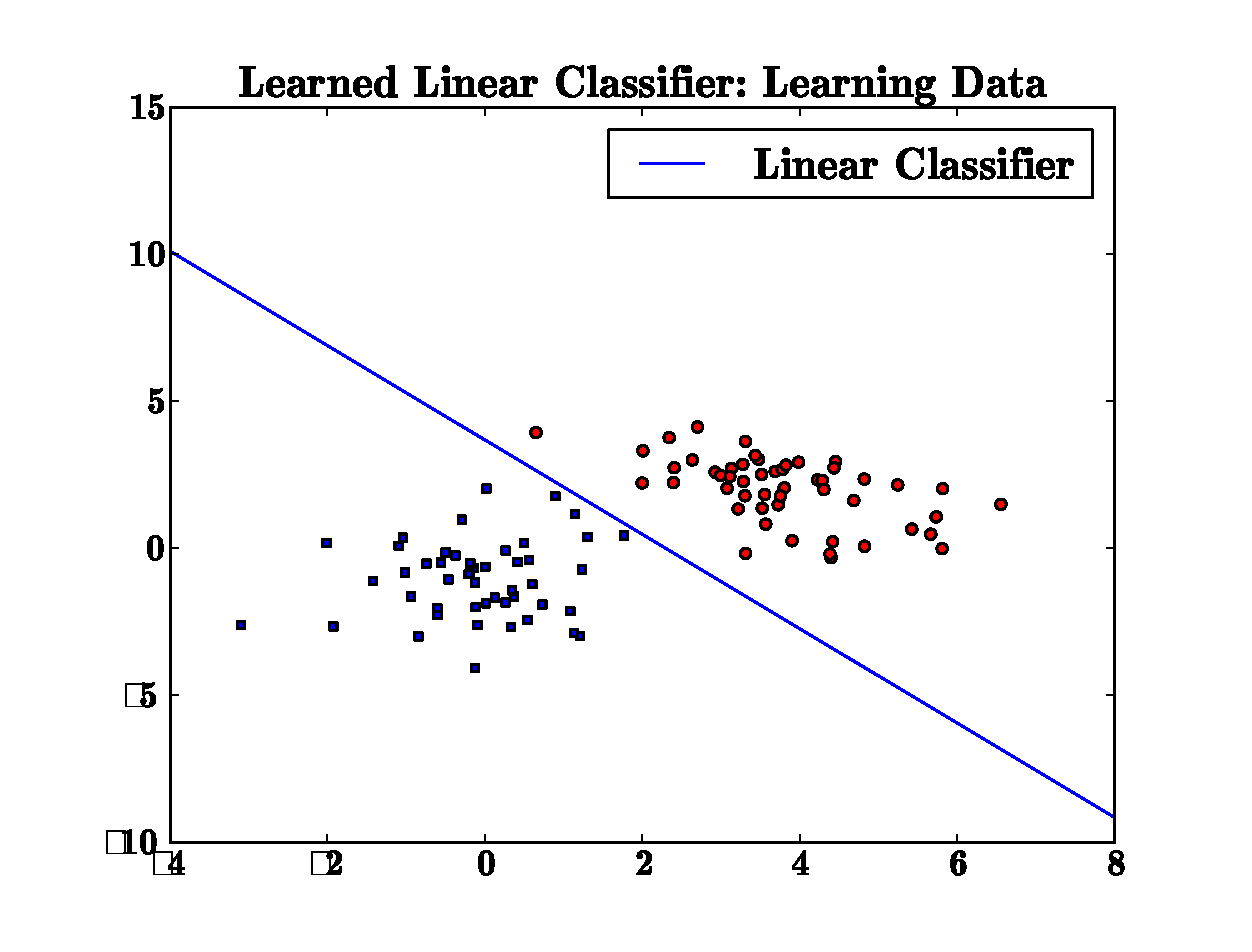
\includegraphics[width=5in]{learn.eps} 
\end{figure} 
\\[5mm]
\begin{figure}[th!]
\centering
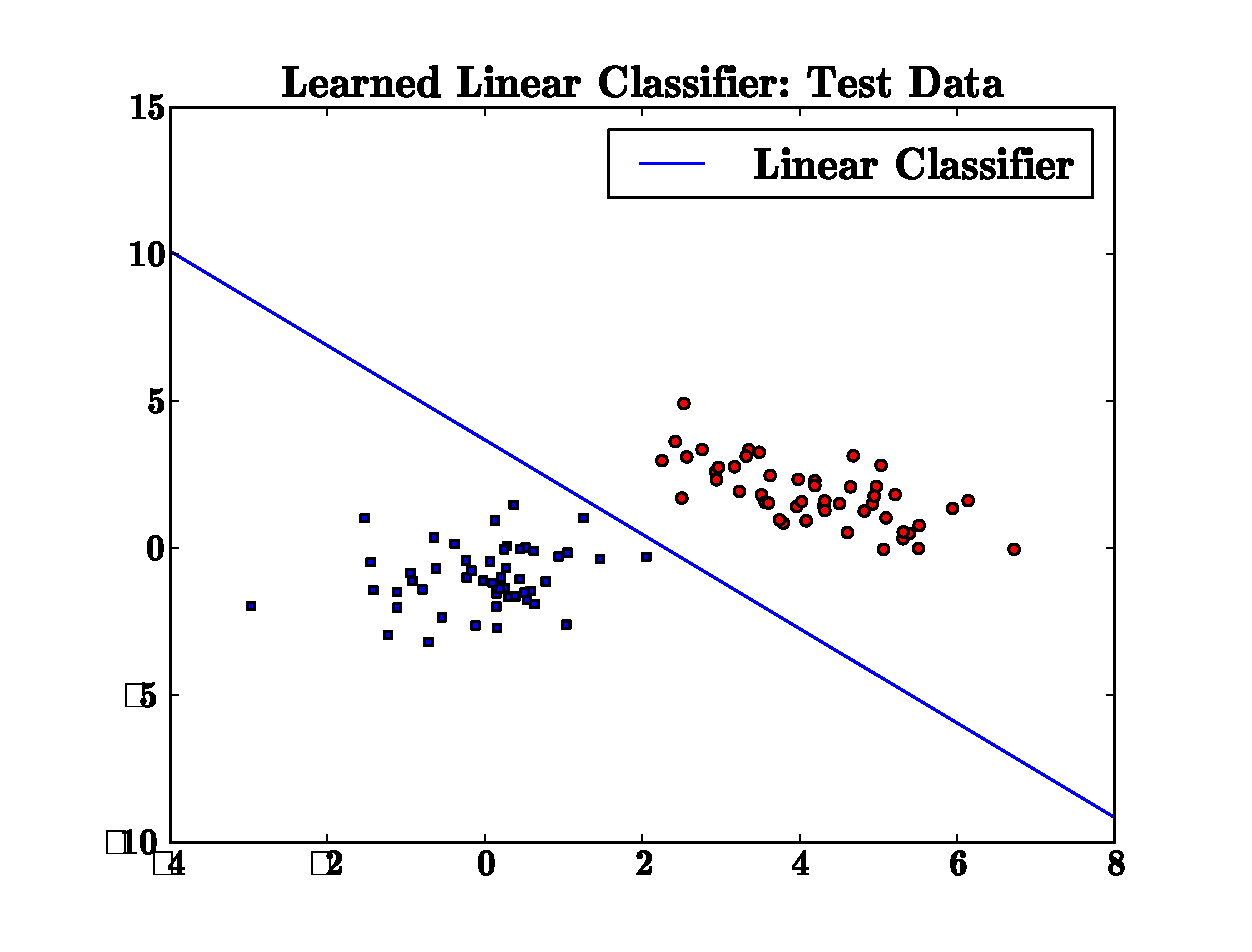
\includegraphics[width=5in]{test.eps} 
\end{figure} 
\\[5mm] 
\pagebreak
\begin{figure}[th!]
\centering
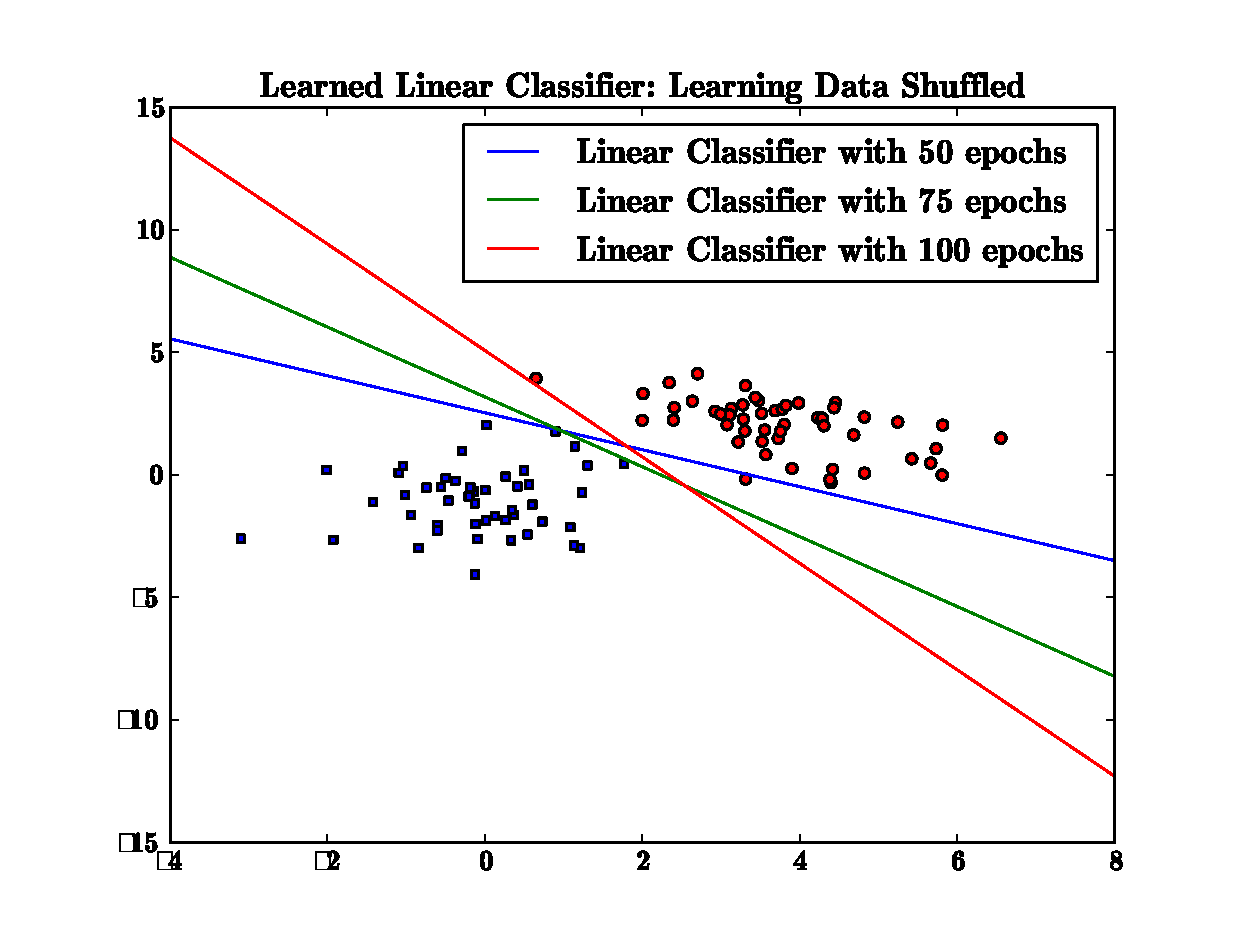
\includegraphics[width=5in]{shuffled.eps} 
\end{figure} 
\\[5mm] 
\begin{figure}[th!]
\centering
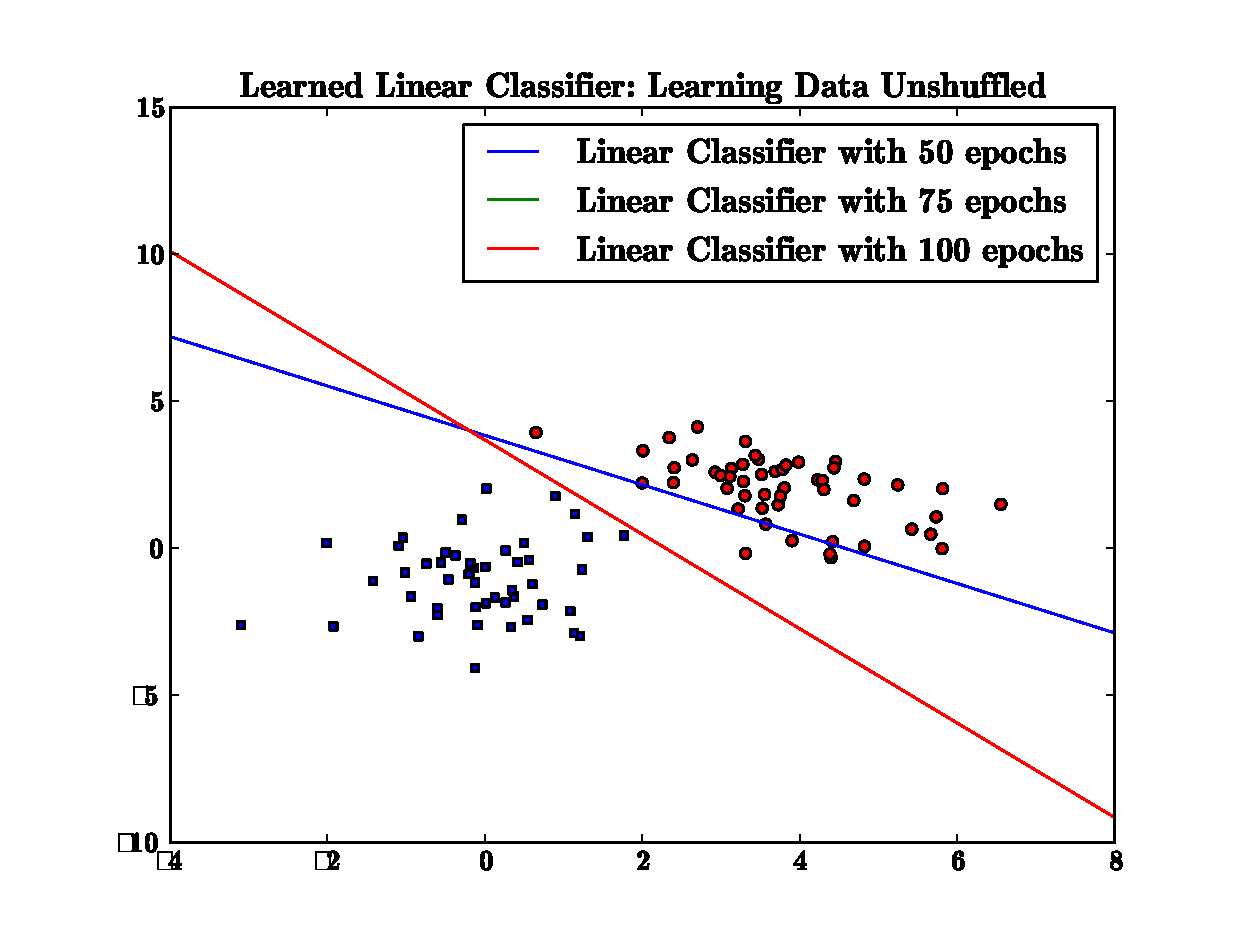
\includegraphics[width=5in]{unshuffled.eps} 
\end{figure} 
\\[5mm]
\pagebreak
\begin{figure}[th!]
\centering
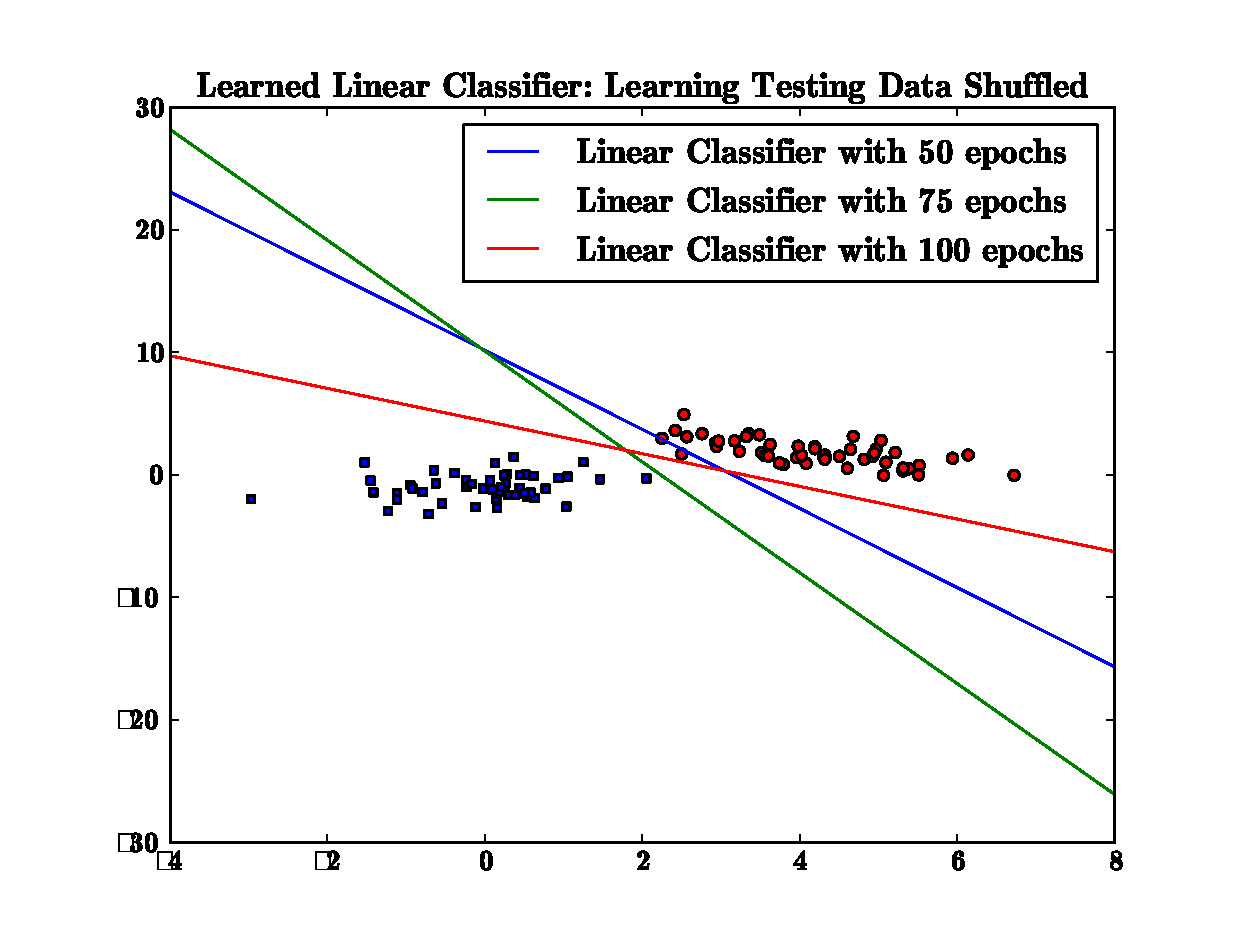
\includegraphics[width=5in]{test_data_shuffled.eps} 
\end{figure} 
\pagebreak
\pagebreak
\begin{figure}[th!]
\centering
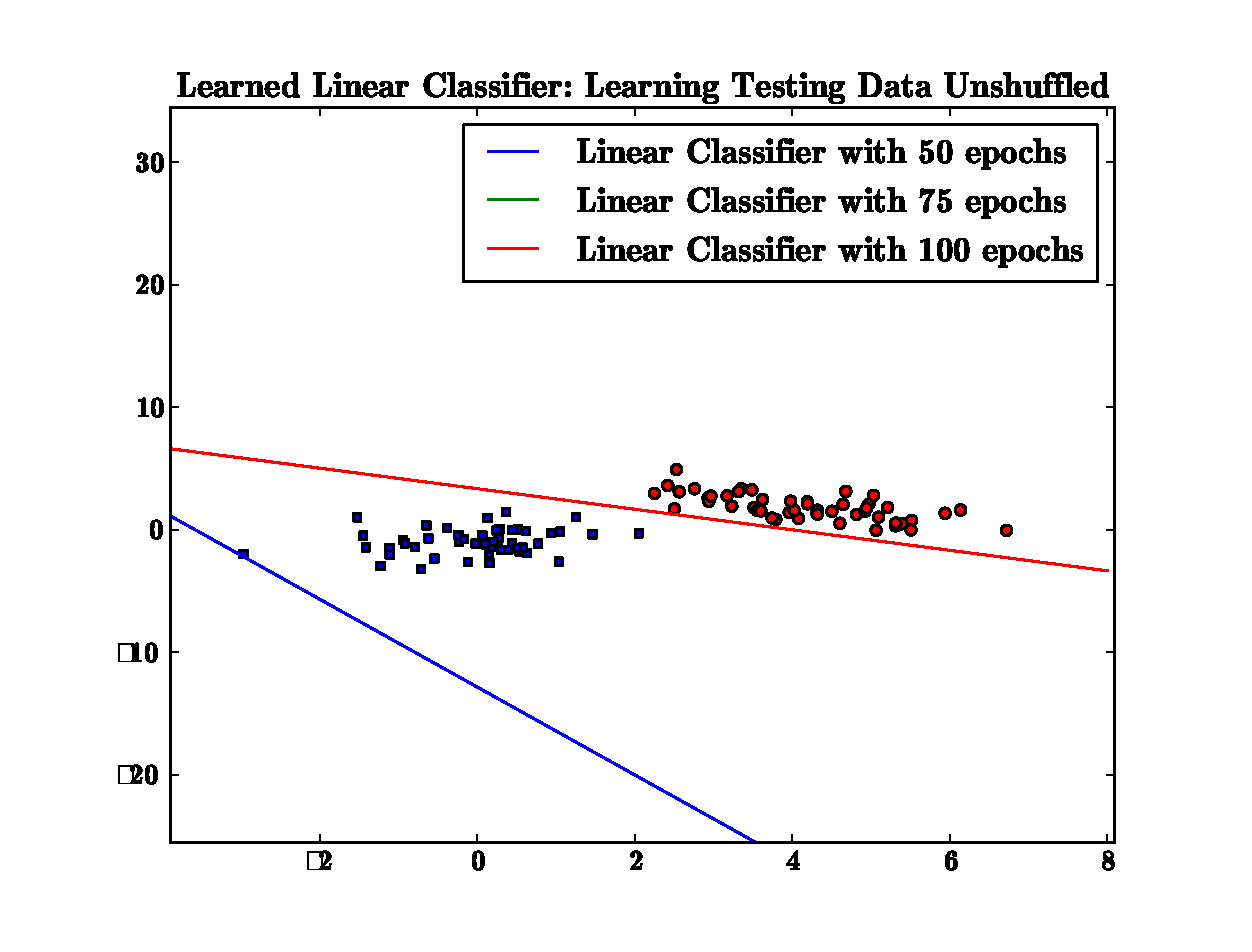
\includegraphics[width=5in]{test_data_unshuffled.eps} 
\end{figure} 
\pagebreak
\\[15mm]
\section{
\\[10mm]
\large \textbf{1. Weather and Traffic Predictions: Supervised Learning} \\[5mm]
Supervised learning algorithms are well suited for problems where there are consistent patterns influenced by one or more independent variables. The algorithms which can solve these problems are relatively easy to understand in that they predict a rate of change given a set of training data. Learning algorithms are most effective when operating on data which is linearly separable. So, it is important that there are definite correlations in our training data. A great application of supervised learning is predicting traffic density based on weather forecast. In order to design an effective solution for this problem we'll first start sampling our training data at uniform intervals. We must agree on quantifiable features which, we suspect, have an effect on our dependent variable. For example, our features could consist of temperature, wind speed, and cloud coverage. These are all valid features which have potential to affect traffic density. To measure the effect we'll also define a threshhold for the traffic density in order to create a classifier. Thus, we have average traffic density act as a linear classifier. A decision tree algorithm would work well for this type of problem due to the relationship between features. For example, there might be an obvious trend in temperature vs. cloud coverage. \\[15mm]

\large 2. \\
a. Using only knee height we find that b $=82.87$ and w1 $= 1.81$ SSE $= 25.879$. \\[5mm]

\begin{figure}[th!]
\centering
\includegraphics[width=5in]{Kneeheight_training.eps} 
\end{figure} 
\\[10mm]
b. Using both of the independent variables we find that the value of b $= 71.315$ and w1 $= .79$, w2 $= .323$ \\
SSE for the arm span is $= 15.93$ \\
\\[5mm]
\begin{tabular}{ | c | c | c | c | c | p{10cm} | }
\hline
Knee Height & Arm Span & Projected & Actual & Error \\ \hline
50.000      & 166.000  & 171.855   & 170.000 & 1.855 \\
57.000      & 196.000  & 187.693   & 191.000 & 3.307 \\
50.000      & 191.000  & 180.442   & 189.000 & 8.558 \\
53.340      & 180.340  & 179.421   & 180.340 & 0.919 \\
54.000      & 174.000  & 177.765   & 171.000 & 6.765 \\
55.880      & 176.530  & 180.120   & 176.530 & 3.590 \\
57.000      & 177.000  & 181.167   & 187.000 & 5.833 \\
55.880      & 208.280  & 191.025   & 185.420 & 5.605 \\
57.000      & 199.000  & 188.723   & 190.000 & 1.277 \\
54.000      & 181.000  & 180.169   & 181.000 & 0.831 \\
55.000      & 178.000  & 179.930   & 180.000 & 0.070 \\
53.000      & 172.000  & 176.288   & 175.000 & 1.288 \\
55.880      & 208.280  & 191.025   & 185.420 & 5.605 \\
57.000      & 199.000  & 188.723   & 190.000 & 1.277 \\
54.000      & 181.000  & 180.169   & 181.000 & 0.831 \\
55.000      & 178.000  & 179.930   & 180.000 & 0.070 \\
53.000      & 172.000  & 176.288   & 175.000 & 1.288 \\
57.000      & 185.000  & 183.915   & 188.000 & 4.085 \\
49.500      & 165.000  & 171.117   & 170.000 & 1.117 \\
57.000      & 188.000  & 184.945   & 185.000 & 0.055 \\ \hline
\end{tabular} 
\\[10mm]
c. The SSE was greater for knee height because of an outlier. Weight might reduce the amount of error gained from the knee height feature as it is less reliable than arm span. \\

\large 3. \\
a. Training error for:  1-nearest neighbor $= 0$ \\
   Leave-one-out error for: 1-nearest neighbor $= 0$ \\
b. Training error for:  3-nearest neighbor $= 3$ \\ 
   Leave-one-out error for: 3-nearest neighbor $3/11$ \\
c. Decision boundary for 1-nearest neighbor \\[5mm]

\begin{figure}[th!]
\centering
\includegraphics[width=5in]{1-neighbor-decision.eps} 
\end{figure} 
 
\\[5mm]

d. I'm assuming the question is asking if the answer will differ from "c" because "a" did not return a subset of lines. The answer is false because the data can't be correctly partitioned  	by drawing a different decision boundary. 


\end{document}
